\chapter{Технологический раздел}
В данном разделе производится выбор средств реализации программного обеспечения, описываются типы и структуры данных, листинги кода, а так же будет продемонстрирован интерфейс программы.

\section{Выбор языка программирования и среды разработки}

Для реализации программного обеспечения был выбран язык C++ по нескольким причинам:
\begin{itemize}
	\item Поддерживает объектно-ориентированную парадигму программирования;
	\item Обладает достаточно высокой производительностью;
	\item Обладает широким набором функций из стандартной библиотеки, в том числе функция замера процессорного времени, которая будет использована в дальнейшем исследовании.
\end{itemize}

В качестве среды разработки был выбран Qt Creator. Он обладает всем необходимым функционалом для написания и отладки программ. Данная среда поставляется с фреймворком Qt, который будет использоваться для создания графического интерфейса программы.


\section{Выбор структур данных}
В данной работе необходимо создать следующие структуры данных:

\begin{enumerate}
	\item Структура, характеризующая перемещение модели;
	\item Структура, характеризующая вращение модели;
	\item Структура, характеризующая масштабирование модели;
	\item Класс, описывающий точку;
	\item Класс, описывающий точки;
	\item Структура, описывающая ребро;
	\item Класс, описывающая ребра;
	\item Структура, описывающая грань;
	\item Класс, описывающий грани;
	\item Класс, описывающий фигуру;
	\item Класс, описывающий отрисовываемое полотно;
	\item Класс, необходимый для взаимодействия пользователя с программой.
\end{enumerate}


\section{Структура программы}
На рисунке~\ref{fig:uml_programm} представлена структура программы в виде UML-диаграммы.

\begin{figure}[H]
	\centering
	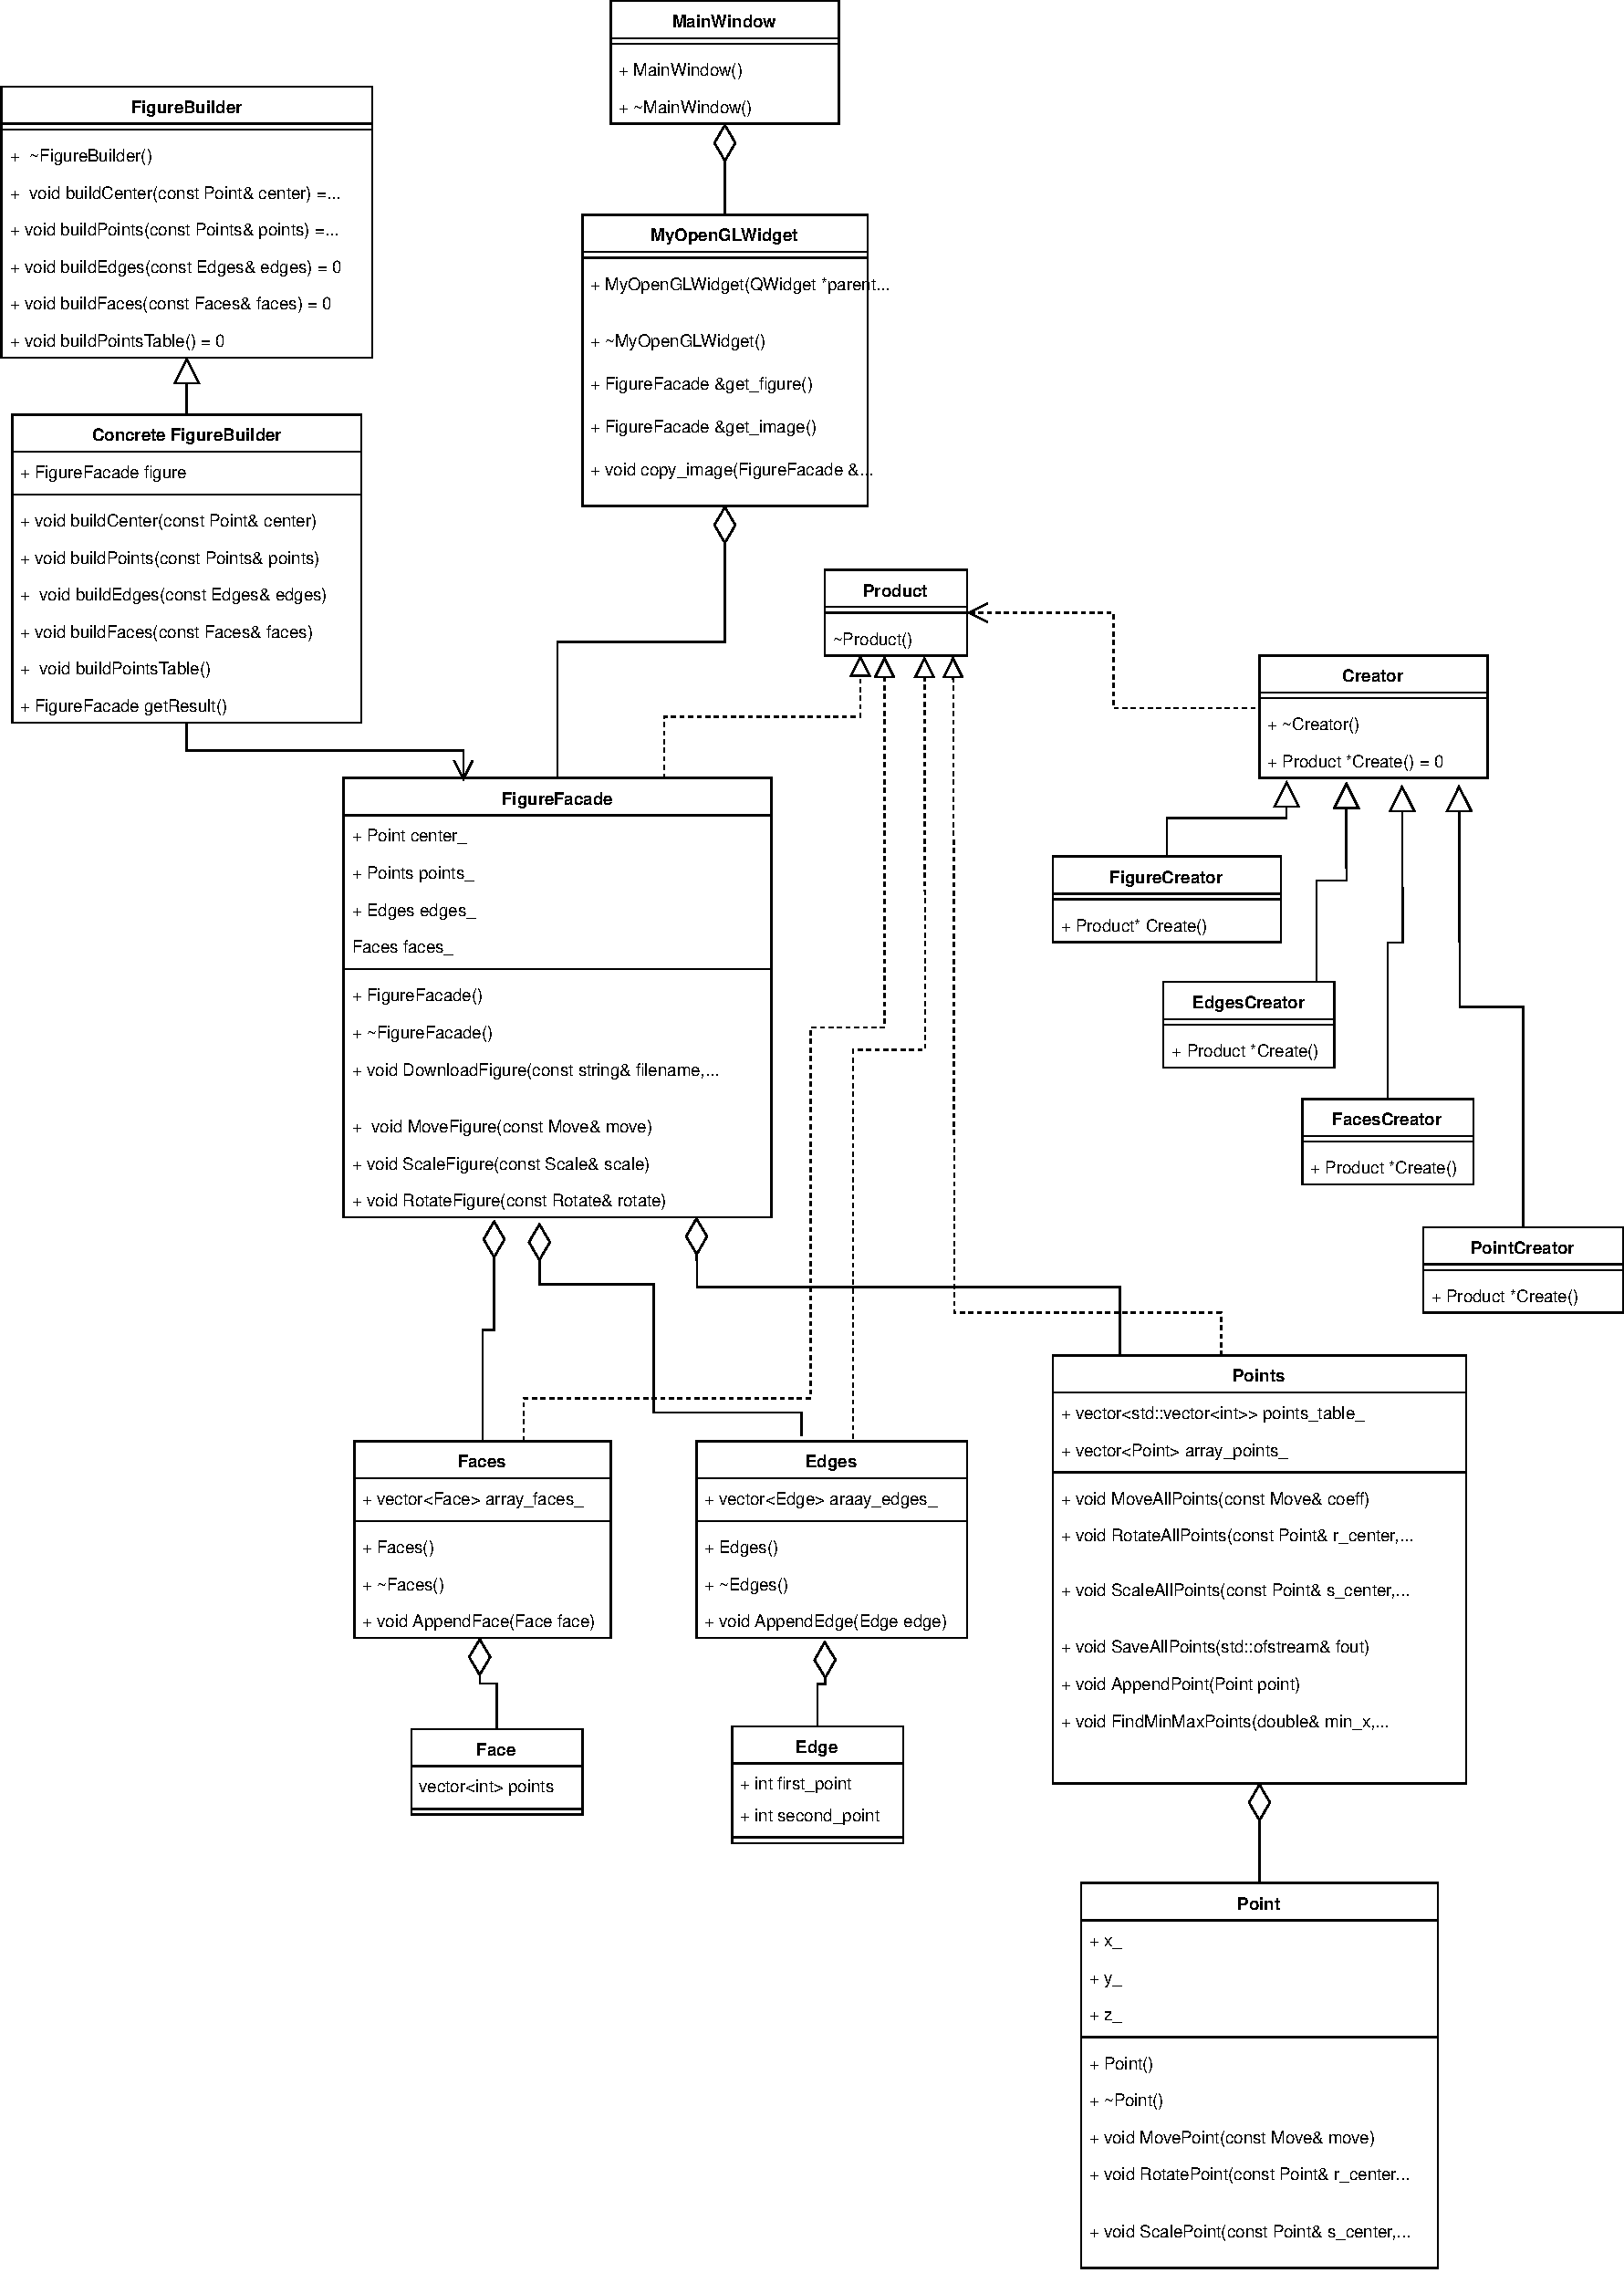
\includegraphics[scale=0.54]{images/programm.pdf}
	\caption{Структура программы}
	\label{fig:uml_programm}
\end{figure}

\newpage

\section{Реализация алгоритмов}
Реализация алгоритма создания фигуры и считывания ее вершин и ребер из .obj файла предоставлена на листингах 3.1-3.6.
Необходимо отметить, что очередное ребро не просто заносится в список. 
Сначала проверяется его наличие (см листинг 3.3 – 3.4). 
Так же для построения фигуры используется паттерн строитель – так код становится логически проще.
За выделение памяти отвечает фабричный метод.


